\PassOptionsToPackage{sols}{handout}
\documentclass[main]{subfiles}
\setcounterrefbeforedot{chapter}{m-ws3-4}
\setcounterrefafterdot{section}{m-ws3-4}
\addtocounter{section}{-1}
\usepackage{solutions}

\begin{document}

\section{Solving Trig Equations} \label{ws3-4}

\begin{problemonly}
    \begin{framed}

\textbf{Key Ideas}:

\begin{itemize}[topsep=0pt,partopsep=0pt,parsep=8pt,itemsep=0pt]

\item You should be able to solve equations involving trigonometric
  functions on both restricted and unrestricted domains.  (In many cases,
  your answers will involve inverse trigonometric functions.) 

\item You should be able to interpret your solutions in the context of a
  problem (for example, what do your solutions tell you about the
  intersections of two graphs?).

\end{itemize}
\end{framed}
\end{problemonly}

\begin{enumerate}
\item 
  \note{Quick motivation for solving trig equations}

  Over the next week, the tides at Pleasant Bay on Cape Cod will be
  roughly periodic, with a period of $12.5$ hours and a $3.8$-foot
  difference between high and low tides.  At 6 am this morning, the water
  was at ``mean sea level'' (half-way between high and low tide), and the
  water level was falling.
  \begin{enumerate}
  \item Which of the following best models the height of the water
    relative to sea level $t$ hours after 6 am?

      \begin{multicols}{2}
      \begin{enumerate}[topsep=0pt,label=\protect\maybecircle{\Alph*.}]
      \plainitem $\displaystyle 1.9 \sin \left(\frac{2\pi}{12.5} t \right)$
      \circleitem $\displaystyle -1.9 \sin \left(\frac{2\pi}{12.5} t \right)$
      \plainitem $\displaystyle 1.9 \cos \left(\frac{2\pi}{12.5} t \right)$
      \plainitem $\displaystyle -1.9 \cos \left(\frac{2\pi}{12.5} t \right)$
      \end{enumerate}
      \end{multicols}
    

    \begin{solution}
      At $t = 0$, the height function is at its mildine value and
      decreasing. 
    \end{solution}
\pspace{-12pt}

  \item
    \note{You might get students to start thinking about domain issues by
      asking them whether $t<0$ is a possibility.}

    \begin{problem}[0.25in]
      There is a causeway at Pleasant Bay that becomes impassable when
      the water is $1.7$ feet above sea level.
      If we want to know the first time after 6 am that the causeway
      will become impassable, what equation do we need to solve?
    \end{problem}

    \begin{solution}
      We want the smallest positive value of $t$ that solves the equation
      $ -1.9 \sin \left(\frac{2\pi}{12.5} t \right) = 1.7$.
    \end{solution}

  \end{enumerate}

\item 
  \note{They've done some problems like this in homework and workshop
    already, but they may still have some trouble.  It's really important
    that students get comfortable solving these ``basic'' equations
    because our strategy for solving more complicated equations is to
    reduce them to these basic ones.} 

  \emph{Solving $\sin x = a$, $\cos x = a$, and $\tan x = a$.}  Solve each
  of the following equations.

  \begin{enumerate}
    \item

    \note{Depending on what strategy students use, solving equations
      involving $\tan$ can feel different because it has period $\pi$.} 

    \begin{problem}[\vfill]
      Find all solutions of $\tan u = -3$.
    \end{problem}

    \begin{solution}
      One solution of $\tan u = -3$ is $\arctan (-3)$; let's call this $A$
      for short.  By definition, it's the angle in $\left( -
        \frac{\pi}{2}, \frac{\pi}{2} \right)$ whose tangent is $-3$.  We
      can visualize $A = \arctan (-3)$ like this:
      \begin{center}
        \begin{tikzangle}[angle=rad(atan(-3)), label=$A$]
          \draw[red] (axis cs: \px, \py) node[anchor=north west, text
          width=1in]{terminal side has slope $-3$};
        \end{tikzangle}
      \end{center}
      When we're solving $\tan u = -3$, we're trying to think of all angles
      whose terminal side has slope $-3$; that's all angles that end on
      either the green or blue segment below:
      \begin{center}
        \begin{tikzangle}[angle=rad(atan(-3)), label=$A$]
          \draw[green!70!black] (axis cs: 0, 0) -- (axis cs: \px, \py);
          \draw[blue] (axis cs: 0, 0) -- (axis cs: \minuspx, \minuspy);
        \end{tikzangle}
      \end{center}
      We can see that such angles are simply $A$ plus an integer multiple
      of $\pi$, so the solutions of $\tan u = -3$ are \fbox{$\pi n +
        \arctan (-3)$ where $n$ is any integer} (that is, $\arctan 2$ plus
      any integer multiple of $\pi$).

      Alternatively, you could think about this in terms of the graph of
      $\tan u$; unlike $\sin$ and $\cos$, $\tan u$ has period $\pi$.  We
      can see from the graph that the solutions of $\tan u = -3$ (marked on
      the $x$-axis in red) are spaced exactly $\pi$ apart:
      \begin{center}
        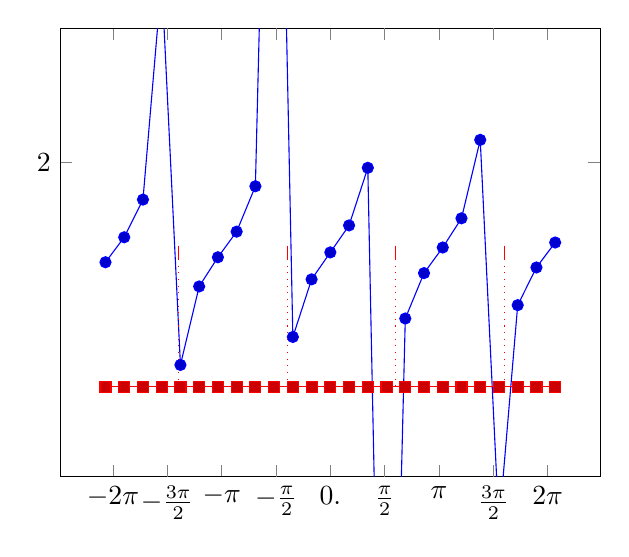
\begin{tikzpicture}
          \begin{axis}[xtick={-6.28319, -3.14159, 0., 3.14159, 6.28319},
            xticklabels={$-2 \pi$, $-\pi$, $0.$, $\pi$, $2 \pi$}, ymin=-5,
            ymax=5, ytick={2}, extra x ticks={-4.71239, -1.5708, 1.5708,
              4.71239}, extra x tick labels={$-\frac{3 \pi }{2}$,
              $-\frac{\pi }{2}$, $\frac{\pi }{2}$, $\frac{3 \pi }{2}$}] %
            \addplot+[domain=-6.5:6.5, restrict y to
            domain=-20:20]{tan(deg(x))}; %
            \addplot+[domain=-6.5:6.5]{-3}; %
            \pgfplotsforeachungrouped \x in {-4.39064, 1.89255, 5.03414,
              -1.24905} %
            {
              \edef\temp{%
                \noexpand\draw[red] (axis cs: \x, 0.15) -- (axis cs:
                \x, -0.15);%
                \noexpand\draw[red, dotted] (axis cs: \x, 0) -- (axis cs:
                \x, -3);% 
              }
              \temp
            }
          \end{axis}          
        \end{tikzpicture}
      \end{center}
    \end{solution}
    
  \item
    \note{Encourage them to think about the graph of $\cos x$; even if
      they don't sketch it, they should see that $[0, 2\pi]$ represents
      1 period of the graph, so the equation should have 2 solutions.}

    \begin{problem}[\vfill\newpage]
      Solve $\cos x = - \frac{1}{2}$ on $[0, 2 \pi]$. 
    \end{problem}

    \begin{solution}
      There are two such angles:
      \begin{center}
        \begin{tikzpicture}
        \begin{axis}[axis equal=true, 
          xmin=-1.2, xmax=1.2, ymin=-1.2, ymax=1.2, clip=false,
          xtick=\empty, ytick=\empty, extra x ticks={-0.5},
          extra x tick style={grid style = {dotted,black}}, width=2.5in]
          \coordinate (O) at (0,0);
          \coordinate (A) at (1,0);
          \coordinate (R) at (\rtheta{1}{120});
          \coordinate (P) at (\rtheta{1}{240});
          \addplot[domain=0:360, data cs=polar] (x,1);
          \draw[thick,blue] (O) -- (R);
          \draw[thick,red] (O) -- (P);
          \filldraw[fill=blue,radius=2pt] (R) circle;
          \filldraw[fill=red,radius=2pt] (P) circle;
          \draw pic[text=blue,draw=blue,thick,angle radius=15,
          "\normalsize$\frac{2\pi}{3}$",angle eccentricity=1.5]
          {angle=A--O--R};
          \draw pic[draw=red,thick,angle radius=10] {angle=A--O--P};
          \draw[->,draw=red,text=red] (-1,0.5) node[left] 
          {\normalsize$\frac{4\pi}{3}$} to (-0.2,0.1);
        \end{axis}
      \end{tikzpicture}
      \end{center}
      The 2 solutions are \fbox{$\frac{2\pi}{3}$ and $\frac{4\pi}{3}$}.
    \end{solution}

  \item

    \begin{problem}[\vfill]
      Solve $\cos u = 0.4$ on $[0, 2 \pi]$.
    \end{problem}

    \begin{solution}
      There are two such angles. Let's express our solutions
      in terms of $A = \arccos(0.4)$, the
      angle in $[0, \pi]$ whose cosine is $0.4$.
     \begin{center}
        \begin{tikzpicture}
        \begin{axis}[axis equal=true, 
          xmin=-1.2, xmax=1.2, ymin=-1.2, ymax=1.2, clip=false,
          xtick=\empty, ytick=\empty, extra x ticks={0.4},
          extra x tick style={grid style = {dotted,black}},width=2.5in]
          \coordinate (O) at (0,0);
          \coordinate (A) at (1,0);
          \coordinate (R) at (\rtheta{1}{66.42});
          \coordinate (P) at (\rtheta{1}{293.58});
          \addplot[domain=0:360, data cs=polar] (x,1);
          \draw[thick,blue] (O) -- (R);
          \draw[thick,red] (O) -- (P);
          \filldraw[fill=blue,radius=2pt] (R) circle;
          \filldraw[fill=red,radius=2pt] (P) circle;
          \draw pic[text=blue,draw=blue,thick,angle radius=15,
          "$A$",angle eccentricity=1.5]
          {angle=A--O--R};
          \draw pic[text=red,draw=red,thick,angle radius=10,
          "$2\pi-A$",angle eccentricity=2.4] {angle=A--O--P};
          % \draw[->,draw=red,text=red] (-1,0.5) node[left] 
          % {\normalsize$\frac{4\pi}{3}$} to (-0.2,0.1);
        \end{axis}
      \end{tikzpicture}
      \end{center}
      That is, the 2 solutions are \fbox{$\arccos(0.4)$ and $2\pi- \arccos(0.4)$}.
    \end{solution}

  \item
    \begin{problem}[\vfill]
      Solve $\cos u = 0.4$ on $[0,4\pi]$.
    \end{problem}

    \begin{solution}
      In addition to the two solutions from part (c), we will have two more solutions
      in $[2\pi,4\pi]$, which we can obtain by adding $2\pi$ to our previous solutions.
      This is because $\cos u$ has a period of $2\pi$.
      
      The 4 solutions are \fbox{$\arccos(0.4)$, $2\pi- \arccos(0.4)$,
      $\arccos(0.4)+2\pi$, and $4\pi-\arccos(0.4)$}.
    \end{solution}

  \item 

  \begin{problem}[\vfill\newpage]
    Solve $\cos(2t)=0.4$ on $[0,2\pi]$.
    
    \emph{Hints: How many solutions do you expect?
      \begin{enumerate}[topsep=0pt]
        \item Begin by substituting $u=2t$.
        \item What is the new interval of interest? When $t=0$, what's $u$?
        When $t=2\pi$, what's $u$?
      \end{enumerate}
      Now you have a new problem all in $u$. Is it the problem you solved in
      part (c) or in part (d)?
    }
    
    \emph{General problem-solving strategy: When a problem is complex,
      substitution can reveal a simpler underlying structure. But caution—you
      must transform the \textbf{entire} problem to the new variable.
    }
  \end{problem}

  \begin{solution}
    Let $u=2t$. When $t=0$, $u=0$, and when $t=2\pi$, $u=4\pi$. Therefore
    we want to solve $\cos u = 0.4$ on $[0,4\pi]$. This is the same as
    part (d), so the solutions are
    \begin{center}
    $u = \arccos(0.4)$, $2\pi-\arccos(0.4)$, $\arccos(0.4)+2\pi$, and 
        $4\pi-\arccos(0.4)$
    \end{center}
        corresponding to
    \begin{center}
    \fbox{$t = \tfrac{1}{2}\arccos(0.4)$, $\pi-\tfrac{1}{2}\arccos(0.4)$, 
        $\tfrac{1}{2}\arccos(0.4) + \pi$, and $2\pi - \tfrac{1}{2}\arccos{0.4}$}
    \end{center}
  \end{solution}

  \item

    \note{The tricky thing here is that $\arcsin (-0.3)$ is \emph{not} one
      of the solutions we want.}

    \begin{problem}[\vfill]
      Solve $\sin t = - 0.3$ on $[0, 4 \pi]$. 
    \end{problem}

    \begin{solution}
      One solution of $\sin t = - 0.3$ is $\arcsin(-0.3)$; let's call this
      $A$ for short.  Remember that $A = \arcsin(-0.3)$ is the angle in
      $\left[ - \frac{\pi}{2}, \frac{\pi}{2} \right]$ whose sine is
      $-0.3$; we can picture it like this:
      \begin{center}
        \begin{tikzangle}[angle=rad(asin(-0.3)), label=$\ A$, color=blue,
          func=sin, functick=$-0.3$] %
          \draw[blue] (axis cs: 1.5, 0) node[right] {$A = \arcsin
            \left(-0.3 \right)$}; 
        \end{tikzangle}
      \end{center}
      (In particular, since $A$ must be in $\left[ - \frac{\pi}{2},
        \frac{\pi}{2} \right]$ and $\sin A$ is negative, $A$ is between
      $-\frac{\pi}{2}$ and $0$.  So, $A$ is \emph{not} one of the
      solutions that we want.)

      Because $A$ is negative, you may find it easier to work in terms of
      $B = \arcsin \left( 0.3 \right)$, which is between $0$ and
      $\frac{\pi}{2}$; we can picture $B$ like this:
      \begin{center}
        \begin{tikzangle}[angle=rad(asin(0.3)), label=$\ B$, color=blue,
          func=sin, functick=$0.3$] %
          \draw[blue] (axis cs: 1.5, 0) node[right] {$B = \arcsin \left(
              0.3 \right)$}; 
        \end{tikzangle}
      \end{center}
      (From our diagrams, we can see that $B = -A$.)

      There are four values of $t$ in $[0, 4 \pi]$ such that $\sin t =
      -0.3$; they're shown below in red:
      \begin{center}
        \begin{tabular}{cccc}
          \begin{tikzangle}[angle=pi+rad(asin(0.3)), label=$t$, func=sin,
            functick=$-0.3$, labelpos=0.55]           
          \end{tikzangle} &
          \begin{tikzangle}[angle=2*pi-rad(asin(0.3)), label=$t$, func=sin,
            functick=$-0.3$, labelpos=0.4]           
          \end{tikzangle} &
          \begin{tikzangle}[angle=3*pi+rad(asin(0.3)), label=$\ t$, func=sin,
            functick=$-0.3$]           
          \end{tikzangle} &
          \begin{tikzangle}[angle=4*pi-rad(asin(0.3)), label=$\ t$, func=sin,
            functick=$-0.3$]           
          \end{tikzangle} \\
          $\displaystyle 
          \begin{aligned}
            t &= \pi + B \\
            &= \pi - A
          \end{aligned}$ & 
          $\displaystyle 
          \begin{aligned}
            t &= 2\pi - B \\
            &= 2\pi + A
          \end{aligned}$ & 
          $\displaystyle 
          \begin{aligned}
            t &= 3\pi + B \\
            &= 3\pi - A
          \end{aligned}$ & 
          $\displaystyle 
          \begin{aligned}
            t &= 4\pi - B \\
            &= 4\pi + A
          \end{aligned}$ 
        \end{tabular}
      \end{center}
      So, there are four solutions, $\boxed{\pi + \arcsin(0.3), 2 \pi -
        \arcsin(0.3), 3 \pi + \arcsin(0.3), 4 \pi - \arcsin(0.3)}$.
      (These can also be expressed as 
      $ \pi - \arcsin(-0.3), 2\pi +\arcsin(-0.3), 3 \pi - \arcsin(-0.3),
      4\pi +\arcsin(-0.3)$.) 
    \end{solution}

  \end{enumerate}

\item  \emph{The joys of substitution.}

  \note{The main thing
    for students to understand is how they can be reduced to solving
    equations of the form $\sin x = a$, $\cos x = a$, or $\tan x = a$.} 

  \begin{enumerate}
  \item

    \note{One confusion students may have is about the two ``types'' of
      substitution; when we substitute for the inside of a trig expression
      (like when we substitute $u = 2t$ to solve $\cos(2t) = 1$), it's
      useful to think about the domain of $u$.  But here, when we're
      substituting for an entire trig expression (like $u = \cos x$), we
      don't need to adjust the domain. Solving part (a)
      both ways will alleviate the confusion.}

    \begin{problem}[\vfill]
      Solve $\dfrac{3}{\cos x +2} = 2$ for $x$ in the interval $[0,2\pi]$. (We can do
      this two ways, with and without substitution.)
    \end{problem}

    \begin{solution}
      First, without substitution. We isolate $\cos x$:
      \begin{align*}
        \frac{3}{\cos x + 2} &= 2 \\
        2(\cos x + 2) &= 3 \\
        \cos x &= -\tfrac{1}{2}
      \end{align*}
      We already solved this equation in \#2(b) and found that the 2 solutions
      are \fbox{$x=\frac{2\pi}{3}$ and $\frac{4\pi}{3}$.}

      Now, with substitution. Let's substitute $u=\cos x$. We then solve for $y$:
      \begin{align*}
        \frac{3}{u + 2} &= 2 \\
        2(u + 2) &= 3 \\
        u &= -\tfrac{1}{2}
      \end{align*}
      Switching back to $x$, we have the same equation $\cos x=-\frac{1}{2}$, with
      the same solutions.
    \end{solution}
    
  \item

    \begin{problem}[\vfill\newpage]
      Solve $2 \cos^2 x + 3 \cos x + 1 = 0$ on $[0, 2\pi]$.
      \emph{Note: This is a quadratic `in $\cos x$'.}
    \end{problem}

    \begin{solution}
      Since the equation involves $\cos x$ in several places (and no other
      $x$'s), let's substitute $u = \cos x$.  The equation becomes
      \begin{align*}
        2u^2 + 3u + 1 &= 0 \\
        (2u + 1)(u + 1) &= 0 \\
        u &= - \frac{1}{2}, -1
      \end{align*}
      So, we now want to solve $\cos x = - \frac{1}{2}$ and $\cos x = -1$
      on $[0,2\pi]$.\footnote{Alternatively, you might have noticed
        right away that the given equation could be factored as $(2 \cos x
        + 1)(\cos x + 1) = 0$.}  This is just like the questions in
      {{\#2}}.  The solutions of $\cos x = - \frac{1}{2}$
      on $[0,2\pi]$ are $\frac{2 \pi}{3}$ and $\frac{5\pi}{3}$,
      while the solution of $\cos x = -1$ on $[0,2\pi]$ is $x =
      \pi$.  So, the solutions of the given equation on $[0,2\pi]$ are
      $\boxed{\pi, \frac{2 \pi}{3}, \frac{5\pi}{3}}$.
    \end{solution}
    
  \end{enumerate}

\item 
  \begin{problem}[\vfill]
    Solve the equation you found in {{{{\#1}}(b)}} to
    find the first time after 6 am that the causeway at Pleasant Bay
    becomes impassable.
  \end{problem}

  \begin{solution}
    We wanted to find the smallest positive value of $t$ such that
    \begin{align*}
      -1.9 \sin \left(\frac{2\pi}{12.5} t \right) &= 1.7 \\
      \intertext{Dividing by $-1.9$,} %
      \sin \left( \frac{2 \pi}{12.5} t \right) &= - \frac{1.7}{1.9} = -
      \frac{17}{19} \\
      \intertext{Let's substitute $u = \frac{2 \pi}{12.5} t$.  Since we're
        interested in values of $t$ with $t > 0$, we want $\frac{2
          \pi}{12.5} t > 0$, and we again want the smallest positive value
        of $u$:} %
      \sin (u) &= - \frac{17}{19} 
    \end{align*}
    Since $\arcsin \left( - \frac{17}{19} \right)$ is negative, I'll
    instead think about this in terms of $B = \arcsin \left( \frac{17}{19}
    \right)$.  Then, the smallest possible value of $u$ such that $\sin(u)
    = - \frac{17}{19}$ is shown below:
    \begin{center}
      \begin{tikzangle}[angle=pi+rad(asin(17/19)),
        secondangle=rad(asin(17/19)), func=sin, functick=$-\frac{17}{19}$,
        secondlabel=$B$, label=$u$, width=2.5in, height=2.5in] 
        \draw[funcline] (axis cs: \qx, \qy) -- (axis cs:
        -\qx, \qy);
        \draw (axis cs: 0, \qy) node[funcxtick] {$\frac{17}{19}$};
      \end{tikzangle}
    \end{center}
    So, the smallest possible value of $u$ such that $\sin(u) = -
    \frac{17}{19}$ is
    \begin{align*}
      u &= \pi + B = \pi + \arcsin \left( \frac{17}{19} \right) \\
      \intertext{Since $u = \frac{2 \pi}{12.5} t$,} %
      t &= \frac{12.5}{2 \pi} u = \boxed{\frac{12.5}{2 \pi} \left( \pi +
          \arcsin \left( \frac{17}{19} \right) \right)} \approx 8.45
    \end{align*}
    So, the first time that the causeway becomes impassable is about 8.45
    hours after 6 am. 
  \end{solution}

\item 

  \note{This is here in a different spirit (and doesn't involve inverse trig.)}

  \begin{problem}[\vfill]
    A felucca (a kind of boat) is sailing up the Nile at a steady pace.
    The river is straight and the felucca maintains a distance of 40 ft from
    the shoreline. At a given moment the boat's bearing to a temple on the shore
    is N \ang{25}E. 5 seconds later, the boat's bearing is N \ang{35}E. How
    fast is the felucca traveling?
    \vspace{-24pt}
  
\includegraphics[scale=0.6]{images/gottlieb-nile.pdf}
  \end{problem}

  \begin{solution}
    To determine the felucca's speed, we should first determine the distance
    it travels in the 5 seconds between observations. Let's call the initial
    and final positions of the boat points $A$ and $B$ respectively. We want to
    find length $AB$. First, let's draw the perpendiculars from $A$ and $B$ to the shoreline. We'll say point $C$ is the position of the temple, and we'll call
    intersections of the perpendiculars from $A$ and $B$ to the shoreline $A'$ and
    $B'$ respectively.
    
    \begin{center}
    \begin{tikzpicture}[scale=0.8]
    \coordinate (A) at (0,0);
    \coordinate (B) at (0,2.865);
    \coordinate (C) at (4,8.579);
    \coordinate (A') at (4,0);
    \coordinate (B') at (4,2.865);
    \filldraw[draw=black,fill=black,radius=2pt] 
      (A) circle node[left] {$A$}
      (B) circle node[left] {$B$}
      (C) circle node[right] {$C$}
      (A') circle node[right] {$A'$}
      (B') circle node[right] {$B'$};
    \draw (A) -- node[below] {40 ft} (A') -- (C) -- cycle;
    \draw (C) -- (B) -- node[below] {40 ft} (B');
    \draw (A) -- (B);
    \draw pic[draw=black,"\ang{65}",angle radius=20] {angle=A'--A--C};
    \draw pic[draw=black,"\ang{55}",angle radius=20] {angle=B'--B--C};
    \draw (A') rectangle (3.4,0.6);
    \draw (B') rectangle (3.4,3.465);
    \end{tikzpicture}
    \end{center}

    Using the headings we are given, we can determine that  $\angle{A'AC}=\ang{65}$
    and $\angle{B'BC}=\ang{55}$. Let's call these angles $\alpha$ and $\beta$ respectively. We also know that $AA'=BB'=40$. Our strategy will
    be to find length $A'B'$ by finding lengths $A'C$ and $A'B'$ and taking the
    difference.

    Consider the two right triangles $AA'C$ and $BB'C$. We want to find the lengths
    of the opposite legs and know the lengths of the adjacent legs, so we can use
    trigonometry:
    \begin{align*}
        A'C &= A'A \tan(\alpha) \quad & B'C &= B'B \tan(\beta) \\
        &= 40 \tan(\ang{65}) &&= 40 \tan(\ang{55}) \\
        &\approx 85.78 &&\approx 57.13
    \end{align*}
    We can then determine that $A'B'=A'C-B'C\approx28.65$.
    
    Therefore the speed at which the felucca is traveling is $\dfrac{28.65\text{ ft}}
    {5\text{ s}}\approx5.7\text{ ft/s}$.
  \end{solution}

\end{enumerate}

\end{document}